\documentclass[12pt,letterpaper,onecolumn,twoside]{article}
%\documentclass[12pt,letterpaper,titlepage,onecolumn,twoside,openright,draft]{book}

% Remove the draft option in order to make the final version of the document

\usepackage{DM_Styles}

% You will see the label just next or above the relevant number in the compiled version.
% Just before the final version, remove it
%\usepackage{showkeys}
%\usepackage{showframe}

% The default font set to sans serif (easy readable)
%\renewcommand*{\familydefault}{\sfdefault}


% Document class options
% 10pt, 11pt, 12pt 	Sets the size of the main font in the document
% a4paper, letterpaper,... Defines the paper size, besides that, a5paper, b5paper, executivepaper, and legalpaper can be specified.
% fleqn 	Typesets displayed formulas left-aligned instead of centered.
% leqno 	Places the numbering of formulas on the left hand side instead of the right.
% titlepage, notitlepage 	Specifies whether a new page should be started after the document title or not.
% onecolumn, twocolumn 	Instructs LaTeX to typeset the document in one column or two columns.
% twoside, oneside 	Specifies whether double or single sided output should be generated. The option twoside does not tell the printer you use that it should actually make a two-sided printout.
% landscape 	Changes the layout of the document to print in landscape mode.
% openright, openany 	Makes chapters begin either only on right hand pages or on the next page available.
% draft 	makes LaTeX indicate hyphenation and justification problems with a small square in the right-hand margin of the problem line so they can be located quickly by a human. It also suppresses the inclusion of images and shows only a frame where they would normally occur.


%%%%%%%%%%%%%%%%%%%%%%%%%%%%%%%%%%%%%%%%%%%%%%%%%%%%%%%%%%%%%
%%%%%%%%%%%%%%%%%%%%%%%%%%%%%%%%%%%%%%%%%%%%%%%%%%%%%%%%%%%%%
%%%                     MAIN DOCUMENT                     %%%
%%%%%%%%%%%%%%%%%%%%%%%%%%%%%%%%%%%%%%%%%%%%%%%%%%%%%%%%%%%%%
%%%%%%%%%%%%%%%%%%%%%%%%%%%%%%%%%%%%%%%%%%%%%%%%%%%%%%%%%%%%%

% \begin{titlepage}
% You can put all of this on a sepparated file and addit by means of
% 
% \begin{document}
% 
%  \input{./title.tex} % This gets the latex code from an external source
%  ...
% \end{document}
% 
%  So you can work with the title in a single file and dont need to recompile
% the whole document


%%% STANDARD TITLE
%%%%%%%%%%%%%%%%%%%%%%%%%%%%%%%%%%%%%%%%

\title{\Huge \scshape \textbf{Sample document showing the use of LatexProjectMakefile} \vspace{1cm} }
\author{ {\large Daniel Mej\'ia Raigosa
  %\thanks{danielmejia55@gmail.com}
} \\ \vspace{1cm} \\ University of Antioquia}
%\date{ \large \today } % actual date
\date{}



%%% HERE THE MAGIC BEGINS
%%%%%%%%%%%%%%%%%%%%%%%%%%%%%%%%%%%%%%%%

\makenomenclature


\begin{document}
%\pagestyle{empty}
\maketitle % if the title is created above
%\include{title-page} % if the title is stored on a sepparated file

%\pagestyle{plain}
\tableofcontents

%\cleardoublepage 
\addcontentsline{toc}{section}{\nomname}
\printnomenclature
%\cleardoublepage 

%\cleardoublepage 
\addcontentsline{toc}{section}{\listfigurename}
%\listoffigures

%\cleardoublepage 
\addcontentsline{toc}{section}{\listtablename}
\listoftables
%\cleardoublepage 

%%\label{ch:list-of-symbols}
\nomenclature{$\frac{\mathrm{d}}{\mathrm{d}x} f\left( x \right)$}{ Derivative of $ f\left( x \right)$}
\nomenclature{$\frac{\mathrm{d}^{2}}{\mathrm{d}x^{2}} f\left( x \right)$}{ Second derivative of $ f\left( x \right)$}

%\label{ch:list-of-symbols}
\nomenclature{$\frac{\mathrm{d}}{\mathrm{d}x} f\left( x \right)$}{ Derivative of $ f\left( x \right)$}
\nomenclature{$\frac{\mathrm{d}^{2}}{\mathrm{d}x^{2}} f\left( x \right)$}{ Second derivative of $ f\left( x \right)$}


%\mainmatter
%% == == == == == == == == == == == == == == == == == == == == == == == == == == == == == == == == == == == == == == == == == ==
%Change header and footer of any page of the document. See DM_Thesis for fancyhdr package

%\newcommand{\changefont}{%
      %\fontsize{8}{9}\selectfont
	%}
%\pagestyle{fancy}
%% First you need to clear the default layout:
%\fancyhf{}
%\fancyfoot[CE,CO]{\thepage}
%\fancyhead[LE]{\changefont \slshape \leftmark}
%\fancyhead[RO]{\changefont \slshape \rightmark}

%% == == == == == == == == == == == == == == == == == == == == == == == == == == == == == == == == == == == == == == == == == ==


\section{\label{ch:introduction} Introduction.}

\subsection{lorem}
Lorem ipsum dolor sit amet, consectetur adipiscing elit. Vivamus interdum tortor libero, in ornare magna imperdiet et. Praesent in vehicula lectus, quis egestas odio. Phasellus pulvinar feugiat elementum. Morbi ac fermentum dui, a suscipit justo. Donec in purus mauris. Vestibulum et tortor est. In pulvinar faucibus tortor, et bibendum odio tincidunt non. Phasellus quis lorem in ex convallis semper.

Nam hendrerit dictum ipsum, a hendrerit enim sollicitudin ac. Pellentesque nulla est, dignissim eget imperdiet vel, rhoncus at ex. Nulla convallis sodales sapien, ut ornare turpis luctus eget. Duis accumsan malesuada turpis, eget eleifend diam. Integer diam libero, molestie scelerisque vehicula in, blandit ut ipsum. Donec libero massa, varius vel tincidunt sit amet, lacinia sit amet neque. Mauris sollicitudin a libero vel fermentum.

Maecenas eu est iaculis turpis finibus mollis. Praesent fringilla semper justo, ut semper enim tincidunt id. Sed molestie mi a sem tincidunt, eu malesuada dolor commodo. Vestibulum ac ex id leo posuere dictum sit amet nec enim. Proin pretium eros in justo porta, sed tempor ex lacinia. Morbi pretium placerat mi, ac facilisis enim suscipit eget. Pellentesque bibendum congue nisl. In suscipit libero sit amet libero pharetra commodo. Duis lacinia ullamcorper ligula, vitae euismod libero gravida nec. Nunc non lectus commodo mi fringilla laoreet in sit amet nulla. Nunc varius felis eros. Maecenas commodo posuere dui at maximus. Sed nec maximus lectus. Mauris id eleifend tortor, ut semper ligula.

\subsection{Cras}
Cras sit amet luctus tellus. Sed eu lacus aliquam, aliquet ipsum in, vestibulum nisl. Aliquam sed vulputate dui. Quisque ullamcorper lorem erat, ut pulvinar nisl ultrices quis. Donec quis sapien faucibus, tempus mi in, rhoncus tellus. Pellentesque id blandit magna. Nam a justo ac erat ultrices vehicula. Quisque sagittis arcu non ante suscipit, a fringilla nulla ullamcorper. Cras vitae eros magna. Phasellus quis dolor ligula.

\subsection{Pallentesque}
Pellentesque urna tortor, volutpat vel elementum in, ullamcorper tristique massa. Etiam et consectetur mi, vel facilisis arcu. Aenean sit amet tincidunt massa. Maecenas cursus molestie ipsum, in bibendum nisl porttitor sit amet. Praesent euismod ipsum et congue convallis. Vivamus eget libero hendrerit, placerat neque eget, condimentum libero. In fringilla vehicula iaculis. Nullam nec lobortis sem, a posuere nisl. Vivamus vulputate vitae turpis in sodales. Integer aliquet augue et libero mattis hendrerit. Sed fringilla sit amet lectus in ornare. Quisque in hendrerit dolor. Donec malesuada lectus orci, in ultricies velit imperdiet non. Ut suscipit nisi nec ex volutpat, vitae consectetur eros ultrices. Praesent aliquam ac libero id gravida. Vestibulum malesuada, tortor eget fringilla ultrices, eros orci tristique metus, a gravida risus lacus a nisl. 

\section{\label{conclusions}Simple chapter.}

\subsection{lorem}
Lorem ipsum dolor sit amet, consectetur adipiscing elit. Vivamus interdum tortor libero, in ornare magna imperdiet et. Praesent in vehicula lectus, quis egestas odio. Phasellus pulvinar feugiat elementum. Morbi ac fermentum dui, a suscipit justo. Donec in purus mauris. Vestibulum et tortor est. In pulvinar faucibus tortor, et bibendum odio tincidunt non. Phasellus quis lorem in ex convallis semper.

Nam hendrerit dictum ipsum, a hendrerit enim sollicitudin ac. Pellentesque nulla est, dignissim eget imperdiet vel, rhoncus at ex. Nulla convallis sodales sapien, ut ornare turpis luctus eget. Duis accumsan malesuada turpis, eget eleifend diam. Integer diam libero, molestie scelerisque vehicula in, blandit ut ipsum. Donec libero massa, varius vel tincidunt sit amet, lacinia sit amet neque. Mauris sollicitudin a libero vel fermentum \cite{Bizzarri2013}.

Maecenas eu est iaculis turpis finibus mollis. Praesent fringilla semper justo, ut semper enim tincidunt id. Sed molestie mi a sem tincidunt, eu malesuada dolor commodo. Vestibulum ac ex id leo posuere dictum sit amet nec enim. Proin pretium eros in justo porta, sed tempor ex lacinia. Morbi pretium placerat mi, ac facilisis enim suscipit eget. Pellentesque bibendum congue nisl. In suscipit libero sit amet libero pharetra commodo. Duis lacinia ullamcorper ligula, vitae euismod libero gravida nec. Nunc non lectus commodo mi fringilla laoreet in sit amet nulla. Nunc varius felis eros. Maecenas commodo posuere dui at maximus. Sed nec maximus lectus. Mauris id eleifend tortor, ut semper ligula.

\begin{figure}[ht]
  \centering
  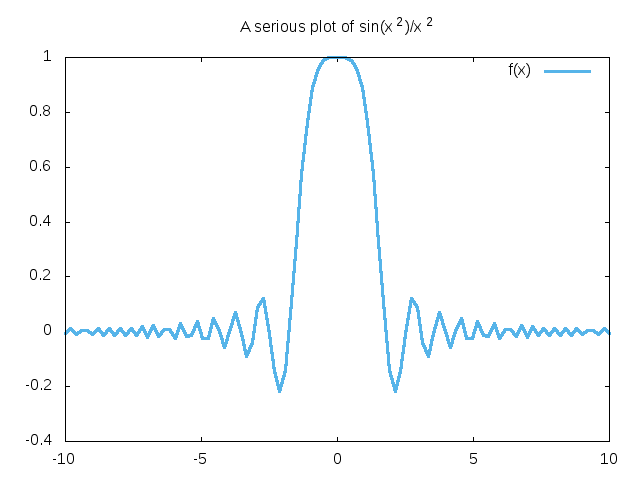
\includegraphics{figures/figure-1}
  \caption{Serious plot of $\sin\left( x^{2} \right)/x^{2}$}
  \label{fig:fig1}
\end{figure}

\subsection{Cras}
Cras sit amet luctus tellus. Sed eu lacus aliquam, aliquet ipsum in, vestibulum nisl. Aliquam sed vulputate dui. Quisque ullamcorper lorem erat, ut pulvinar nisl ultrices quis. Donec quis sapien faucibus, tempus mi in, rhoncus tellus. Pellentesque id blandit magna. Nam a justo ac erat ultrices vehicula. Quisque sagittis arcu non ante suscipit, a fringilla nulla ullamcorper. Cras vitae eros magna. Phasellus quis dolor ligula \cite{Bizzarri2013}.

\subsection{Pallentesque}
Pellentesque urna tortor, volutpat vel elementum in, ullamcorper tristique massa. Etiam et consectetur mi, vel facilisis arcu. Aenean sit amet tincidunt massa. Maecenas cursus molestie ipsum, in bibendum nisl porttitor sit amet. Praesent euismod ipsum et congue convallis. Vivamus eget libero hendrerit, placerat neque eget, condimentum libero. In fringilla vehicula iaculis. Nullam nec lobortis sem, a posuere nisl. Vivamus vulputate vitae turpis in sodales. Integer aliquet augue et libero mattis hendrerit. Sed fringilla sit amet lectus in ornare. Quisque in hendrerit dolor. Donec malesuada lectus orci, in ultricies velit imperdiet non. Ut suscipit nisi nec ex volutpat, vitae consectetur eros ultrices. Praesent aliquam ac libero id gravida. Vestibulum malesuada, tortor eget fringilla ultrices, eros orci tristique metus, a gravida risus lacus a nisl. 

\chapter{\label{ch:complex_chapter}Complex Chapter.}


\subsection{\label{ch:sec:complex-sec}Complex section}


Lorem ipsum dolor sit amet, consectetur adipiscing elit. Vivamus interdum tortor libero, in ornare magna imperdiet et. Praesent in vehicula lectus, quis egestas odio. Phasellus pulvinar feugiat elementum. Morbi ac fermentum dui, a suscipit justo. Donec in purus mauris. Vestibulum et tortor est. In pulvinar faucibus tortor, et bibendum odio tincidunt non. Phasellus quis lorem in ex convallis semper.

Nam hendrerit dictum ipsum, a hendrerit enim sollicitudin ac. Pellentesque nulla est, dignissim eget imperdiet vel, rhoncus at ex. Nulla convallis sodales sapien, ut ornare turpis luctus eget. Duis accumsan malesuada turpis, eget eleifend diam. Integer diam libero, molestie scelerisque vehicula in, blandit ut ipsum. Donec libero massa, varius vel tincidunt sit amet, lacinia sit amet neque. Mauris sollicitudin a libero vel fermentum.

Maecenas eu est iaculis turpis finibus mollis. Praesent fringilla semper justo, ut semper enim tincidunt id. Sed molestie mi a sem tincidunt, eu malesuada dolor commodo. Vestibulum ac ex id leo posuere dictum sit amet nec enim. Proin pretium eros in justo porta, sed tempor ex lacinia. Morbi pretium placerat mi, ac facilisis enim suscipit eget. Pellentesque bibendum congue nisl. In suscipit libero sit amet libero pharetra commodo. Duis lacinia ullamcorper ligula, vitae euismod libero gravida nec. Nunc non lectus commodo mi fringilla laoreet in sit amet nulla. Nunc varius felis eros. Maecenas commodo posuere dui at maximus. Sed nec maximus lectus. Mauris id eleifend tortor, ut semper ligula \cite{Melham2013}.

\begin{table}[!h]
  \centering
  \begin{tabular}{l|r}
	%\hline
	\tableHead
	\multicolumn{2}{c}{\textbf{This is a table}}\\
	\tableTopLine
	%\hline \hline
	\textbf{A column} &\textbf{Another column}\\
	\hline
	I'm a field & I'm the contents \\ \hline
	I'm a field & I'm the contents \\ \hline
	I'm a field & I'm the contents \\ \hline
	I'm a field & I'm the contents \\
\tableBottomLine
	%\hline
	%\hline
\end{tabular}
\caption{\textbf{This is a seriuous table} showing how tables work and such.  \label{tab:table}}
\end{table}




Cras sit amet luctus tellus. Sed eu lacus aliquam, aliquet ipsum in, vestibulum nisl. Aliquam sed vulputate dui. Quisque ullamcorper lorem erat, ut pulvinar nisl ultrices quis. Donec quis sapien faucibus, tempus mi in, rhoncus tellus. Pellentesque id blandit magna. Nam a justo ac erat ultrices vehicula. Quisque sagittis arcu non ante suscipit, a fringilla nulla ullamcorper. Cras vitae eros magna. Phasellus quis dolor ligula.

Pellentesque urna tortor, volutpat vel elementum in, ullamcorper tristique massa. Etiam et consectetur mi, vel facilisis arcu. Aenean sit amet tincidunt massa. Maecenas cursus molestie ipsum, in bibendum nisl porttitor sit amet. Praesent euismod ipsum et congue convallis. Vivamus eget libero hendrerit, placerat neque eget, condimentum libero. In fringilla vehicula iaculis. Nullam nec lobortis sem, a posuere nisl. Vivamus vulputate vitae turpis in sodales. Integer aliquet augue et libero mattis hendrerit. Sed fringilla sit amet lectus in ornare. Quisque in hendrerit dolor. Donec malesuada lectus orci, in ultricies velit imperdiet non. Ut suscipit nisi nec ex volutpat, vitae consectetur eros ultrices. Praesent aliquam ac libero id gravida. Vestibulum malesuada, tortor eget fringilla ultrices, eros orci tristique metus, a gravida risus lacus a nisl \cite{Melham2013}. 



\subsection{\label{ch:sec:complex-sec2}Second complex section}


Lorem ipsum dolor sit amet, consectetur adipiscing elit. Vivamus interdum tortor libero, in ornare magna imperdiet et. Praesent in vehicula lectus, quis egestas odio. Phasellus pulvinar feugiat elementum. Morbi ac fermentum dui, a suscipit justo. Donec in purus mauris. Vestibulum et tortor est. In pulvinar faucibus tortor, et bibendum odio tincidunt non. Phasellus quis lorem in ex convallis semper.

Nam hendrerit dictum ipsum, a hendrerit enim sollicitudin ac. Pellentesque nulla est, dignissim eget imperdiet vel, rhoncus at ex. Nulla convallis sodales sapien, ut ornare turpis luctus eget. Duis accumsan malesuada turpis, eget eleifend diam. Integer diam libero, molestie scelerisque vehicula in, blandit ut ipsum. Donec libero massa, varius vel tincidunt sit amet, lacinia sit amet neque. Mauris sollicitudin a libero vel fermentum.

Maecenas eu est iaculis turpis finibus mollis. Praesent fringilla semper justo, ut semper enim tincidunt id. Sed molestie mi a sem tincidunt, eu malesuada dolor commodo. Vestibulum ac ex id leo posuere dictum sit amet nec enim. Proin pretium eros in justo porta, sed tempor ex lacinia. Morbi pretium placerat mi, ac facilisis enim suscipit eget. Pellentesque bibendum congue nisl. In suscipit libero sit amet libero pharetra commodo. Duis lacinia ullamcorper ligula, vitae euismod libero gravida nec. Nunc non lectus commodo mi fringilla laoreet in sit amet nulla. Nunc varius felis eros. Maecenas commodo posuere dui at maximus. Sed nec maximus lectus. Mauris id eleifend tortor, ut semper ligula.

Cras sit amet luctus tellus. Sed eu lacus aliquam, aliquet ipsum in, vestibulum nisl. Aliquam sed vulputate dui. Quisque ullamcorper lorem erat, ut pulvinar nisl ultrices quis. Donec quis sapien faucibus, tempus mi in, rhoncus tellus. Pellentesque id blandit magna. Nam a justo ac erat ultrices vehicula. Quisque sagittis arcu non ante suscipit, a fringilla nulla ullamcorper. Cras vitae eros magna. Phasellus quis dolor ligula.

Pellentesque urna tortor, volutpat vel elementum in, ullamcorper tristique massa. Etiam et consectetur mi, vel facilisis arcu. Aenean sit amet tincidunt massa. Maecenas cursus molestie ipsum, in bibendum nisl porttitor sit amet. Praesent euismod ipsum et congue convallis. Vivamus eget libero hendrerit, placerat neque eget, condimentum libero. In fringilla vehicula iaculis. Nullam nec lobortis sem, a posuere nisl. Vivamus vulputate vitae turpis in sodales. Integer aliquet augue et libero mattis hendrerit. Sed fringilla sit amet lectus in ornare. Quisque in hendrerit dolor. Donec malesuada lectus orci, in ultricies velit imperdiet non. Ut suscipit nisi nec ex volutpat, vitae consectetur eros ultrices. Praesent aliquam ac libero id gravida. Vestibulum malesuada, tortor eget fringilla ultrices, eros orci tristique metus, a gravida risus lacus a nisl. 




\section{\label{ch:appendices}Appendices.}

\section{\label{ch:appendix:apx1} Appendix.}

\section{lorem}
Lorem ipsum dolor sit amet, consectetur adipiscing elit. Vivamus interdum tortor libero, in ornare magna imperdiet et. Praesent in vehicula lectus, quis egestas odio. Phasellus pulvinar feugiat elementum. Morbi ac fermentum dui, a suscipit justo. Donec in purus mauris. Vestibulum et tortor est. In pulvinar faucibus tortor, et bibendum odio tincidunt non. Phasellus quis lorem in ex convallis semper.

Nam hendrerit dictum ipsum, a hendrerit enim sollicitudin ac. Pellentesque nulla est, dignissim eget imperdiet vel, rhoncus at ex. Nulla convallis sodales sapien, ut ornare turpis luctus eget. Duis accumsan malesuada turpis, eget eleifend diam. Integer diam libero, molestie scelerisque vehicula in, blandit ut ipsum. Donec libero massa, varius vel tincidunt sit amet, lacinia sit amet neque. Mauris sollicitudin a libero vel fermentum.

Maecenas eu est iaculis turpis finibus mollis. Praesent fringilla semper justo, ut semper enim tincidunt id. Sed molestie mi a sem tincidunt, eu malesuada dolor commodo. Vestibulum ac ex id leo posuere dictum sit amet nec enim. Proin pretium eros in justo porta, sed tempor ex lacinia. Morbi pretium placerat mi, ac facilisis enim suscipit eget. Pellentesque bibendum congue nisl. In suscipit libero sit amet libero pharetra commodo. Duis lacinia ullamcorper ligula, vitae euismod libero gravida nec. Nunc non lectus commodo mi fringilla laoreet in sit amet nulla. Nunc varius felis eros. Maecenas commodo posuere dui at maximus. Sed nec maximus lectus. Mauris id eleifend tortor, ut semper ligula.

\section{Cras}
Cras sit amet luctus tellus. Sed eu lacus aliquam, aliquet ipsum in, vestibulum nisl. Aliquam sed vulputate dui. Quisque ullamcorper lorem erat, ut pulvinar nisl ultrices quis. Donec quis sapien faucibus, tempus mi in, rhoncus tellus. Pellentesque id blandit magna. Nam a justo ac erat ultrices vehicula. Quisque sagittis arcu non ante suscipit, a fringilla nulla ullamcorper. Cras vitae eros magna. Phasellus quis dolor ligula.

\subsection{Pallentesque}
Pellentesque urna tortor, volutpat vel elementum in, ullamcorper tristique massa. Etiam et consectetur mi, vel facilisis arcu. Aenean sit amet tincidunt massa. Maecenas cursus molestie ipsum, in bibendum nisl porttitor sit amet. Praesent euismod ipsum et congue convallis. Vivamus eget libero hendrerit, placerat neque eget, condimentum libero. In fringilla vehicula iaculis. Nullam nec lobortis sem, a posuere nisl. Vivamus vulputate vitae turpis in sodales. Integer aliquet augue et libero mattis hendrerit. Sed fringilla sit amet lectus in ornare. Quisque in hendrerit dolor. Donec malesuada lectus orci, in ultricies velit imperdiet non. Ut suscipit nisi nec ex volutpat, vitae consectetur eros ultrices. Praesent aliquam ac libero id gravida. Vestibulum malesuada, tortor eget fringilla ultrices, eros orci tristique metus, a gravida risus lacus a nisl. 




\addcontentsline{toc}{section}{References}
\renewcommand\bibname{References}
\bibliographystyle{apa}
\bibliography{references/references}{}

\end{document}
